%!TEX root = ../SzFDR_jegyzet_v3.tex
\chapter{Ismétlés: folytonos dinamikai rendszerek kvalitatív elmélete}

Tekintsük az $\dot{x}=f(x)$ dinamikai rendszert, ahol $x \in \mathcal{D} \subset \mathbb{R}^n$ és $\mathcal{D}$ az értelmezési tartomány. Legyen $\Phi(x,t)$ a megoldásoperátor (flow), amely az $x$ kezdeti értéket a $t$-beli megoldásba viszi át:
\[
\frac{\partial}{\partial t} \Phi(x,t)=f(\Phi(x,t)), \quad \Phi(x,0)=x.
\]
Ha $f\in C^r$ ($r\geq1$), a lokális megoldásoperátor a kezdeti állapot és az idő együttes függvényeként $C^r$ simaságú. Az idő szerinti deriválhatóságot és a kezdeti állapot szerinti simaságot meg kell különböztetni; általában nincs egyfokú simaságnövekedés az összes változóban.

Az explicit időfüggő $\dot{x}=f(x,t)$ rendszert az $s=t$ állapot bevezetésével autonómmá tehetjük:
\[
\dot{x}=f(x,s),\qquad \dot{s}=1,\qquad
D_{(x,s)}\begin{pmatrix}f(x,s)\\1\end{pmatrix}
=\begin{pmatrix}f_x&f_s\\0&0\end{pmatrix}.
\]
A Jacobi-mátrix utolsó sora nulla; az utolsó oszlop általában nem nulla. A kibővített rendszernek $\dot{s}=1$ miatt nincs egyensúlyi helyzete. Periodikus gerjesztésnél $s$ a gerjesztés periódusa szerint értelmezett fázisváltozóként kezelhető. Az így kapott autonóm rendszer periodikus pályájának időeltolási irányához egységnyi Floquet-multiplikátor tartozik; ez nem a Jacobi-mátrix $1$ sajátértékét jelenti. A gerjesztés rögzített fázisában vett stroboszkopikus leképezés ezt a fázisirányt nem tartalmazza.

Egy \emph{leképezésnek}  a
\[
x\mapsto f(x)
\]
szabályt nevezzük, ahol $x \in \mathcal{D} \subset \mathbb{R}^n$. A szabályt $m$-szer alkalmazva $x_m=f^m(x_0)$, ahol a felső index itt iterációt, nem deriválást jelöl. Ezeket a rendszereket szokás az ún. cobweb diagramon ábrázolni, ahol $x_{n+1}$-et $x_n$ függvényében ábrázoljuk.

\emph{Invariáns halmaznak} egy olyan $\Lambda \subset \mathcal{D}$ részhalmazt nevezünk, hogy ha $x_0 \in \Lambda$ akkor $\Phi(x_0,t) \in \Lambda$ minden t-re. Például egyensúlyi helyzet, illetve periodikus pálya, melyek természetesen lehetnek stabilak vagy instabilak.

A dinamikai rendszereink gyakran függeni fognak valamilyen paraméterektől, ezért gyakran írjuk fel ezeket $\dot{x}=f(x,\mu)$ alakban, ahol $\mu \in \mathbb{R}^p$ a paramétervektor.

\section{Egyensúlyi helyzet}\label{sec:equilibria}
Az $\dot x=f(x)$ autonóm rendszer \emph{egyensúlyi helyzete} olyan $x^*$ pont, amelyre $f(x^*)=0$. Ha innen indulunk, $x(t)=x^*$ minden időben. A stabilitás kérdése az, hogy mi történik egy kicsiny kezdeti eltérés után: a mozgás a pont közelében marad, visszatér hozzá, vagy eltávolodik tőle? Először kétdimenziós lineáris példákon szemléltetjük a geometriát, majd általánosítunk $N$ dimenzióra. A háttérhez lásd di Bernardo és szerzőtársai \cite[2.1.1., 2.1.3--2.1.4. szakasz]{dib}, valamint Kuznetsov \cite[1.3.3. és 2.2.1. szakasz]{kuznetsov_book}.

\subsection{Kétdimenziós fázisportrék: nyereg, csomó és fókusz}
Legyen $y=(y_1,y_2)^\mathsf T$ az egyensúlytól mért eltérés, és tekintsük a $\dot y=Ay$ rendszert. A \emph{fázisportré} az állapotsíkban ábrázolt megoldásgörbék és időirányuk együttese. Az alábbi ábrák saját készítésű, konkrét lineáris rendszerekhez tartozó portrék. A nyilak a növekvő idő irányát mutatják; a görbék sűrűsége és a nyilak hossza nem a sebesség nagyságát kódolja. Az osztályozás megfelel Kuznetsov \cite[2.2.1. szakasz, 2.3. példa és 2.5. ábra]{kuznetsov_book} felosztásának.

\paragraph*{Nyeregpont.}
A legegyszerűbb példa
\begin{equation}\label{eq:planar_saddle}
A=\begin{pmatrix}-1&0\\0&1\end{pmatrix},\qquad
\dot y_1=-y_1,\quad \dot y_2=y_2,
\end{equation}
amelynek megoldása $y_1(t)=y_1(0)e^{-t}$, $y_2(t)=y_2(0)e^t$. A $y_2=0$ egyenes mentén a pályák az origóhoz tartanak: ez a stabil sajátirány. A $y_1=0$ egyenes az instabil sajátirány, rajta a mozgás kifelé halad. A többi pálya eleinte közeledhet az origóhoz, de végül eltávolodik tőle. Emiatt a nyereg \emph{instabil}, noha létezik hozzá tartó pályacsalád. A tengelyeken kívül $y_1y_2$ állandó, ezért a pályák hiperbolaágak.
\begin{figure}[!htbp]\centering
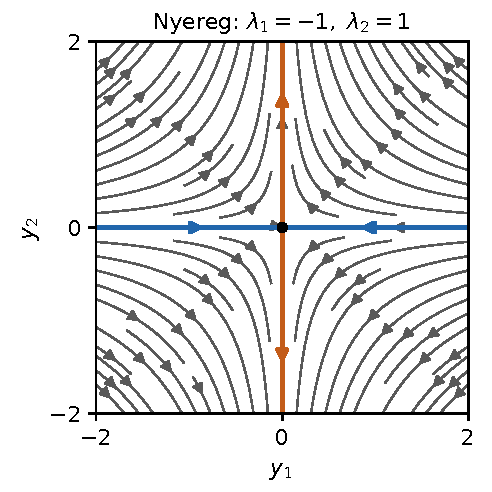
\includegraphics[width=.52\linewidth]{graphics_v3/phase_saddle.pdf}
\caption{Nyeregpont: $\lambda_1=-1$, $\lambda_2=1$. Kék egyenes: stabil irány; narancssárga egyenes: instabil irány. Az origó fekete pont.}\label{fig:phase_saddle}
\end{figure}

\paragraph*{Stabil és instabil csomópont.}
Az $A=\operatorname{diag}(-1,-2)$ mátrix esetén mindkét sajátérték negatív:
\[
y_1(t)=y_1(0)e^{-t},\qquad y_2(t)=y_2(0)e^{-2t}.
\]
Minden pálya az origóhoz tart. A második komponens gyorsabban csökken, ezért az általános pályák a lassabb, $y_1$ sajátirányhoz simulnak. Kivétel a tisztán gyors sajátirányon induló pálya. Az $A=\operatorname{diag}(1,2)$ rendszerben mindkét komponens növekszik: az origó instabil csomópont. A két ábra görbéi azonosak, az időirány ellentétes.
\begin{figure}[!htbp]\centering
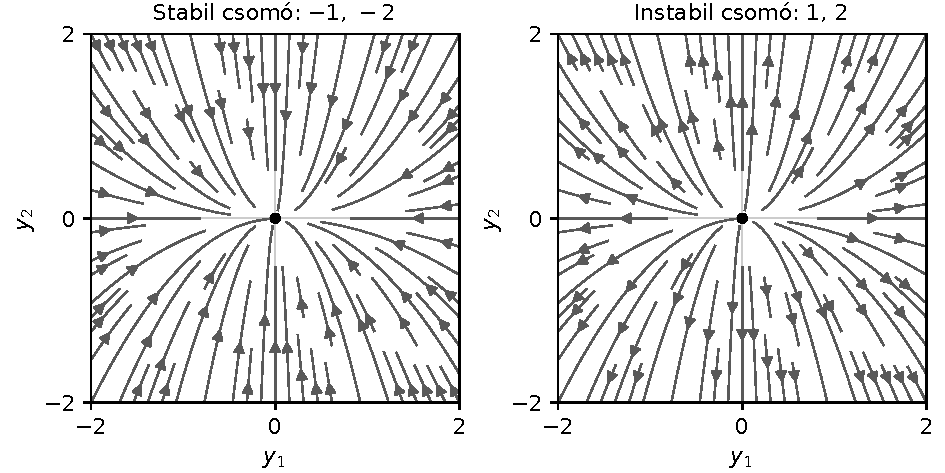
\includegraphics[width=\linewidth]{graphics_v3/phase_nodes.pdf}
\caption{Csomópontok. Balra $A=\operatorname{diag}(-1,-2)$: stabil; jobbra $A=\operatorname{diag}(1,2)$: instabil. A sajátirányokon egyenes, a többi kezdeti állapotból görbült pályát kapunk.}\label{fig:phase_nodes}
\end{figure}

\paragraph*{Stabil és instabil fókusz.}
Komplex konjugált sajátértékpárhoz valós koordinátákban a
\begin{equation}\label{eq:focus_block}
A=\begin{pmatrix}\alpha&-\beta\\\beta&\alpha\end{pmatrix},\qquad
\lambda_{1,2}=\alpha\pm i\beta,\quad \beta\neq0
\end{equation}
blokk tartozhat. A $y_1=\rho\cos\theta$, $y_2=\rho\sin\theta$ polárkoordinátákkal
\begin{equation}\label{eq:focus_polar}
\dot\rho=\alpha\rho,\qquad \dot\theta=\beta,\qquad
\rho(t)=\rho(0)e^{\alpha t}.
\end{equation}
A $\beta$ a forgást, $\alpha$ a spirál összehúzódását vagy tágulását szabályozza. $\alpha<0$ esetén stabil, $\alpha>0$ esetén instabil fókuszt kapunk. A \ref{fig:phase_foci}. ábrán $\beta=1$, ezért mindkét esetben az óramutató járásával ellentétes a forgás; csak a sugár időbeli változása különbözik.
\begin{figure}[!htbp]\centering
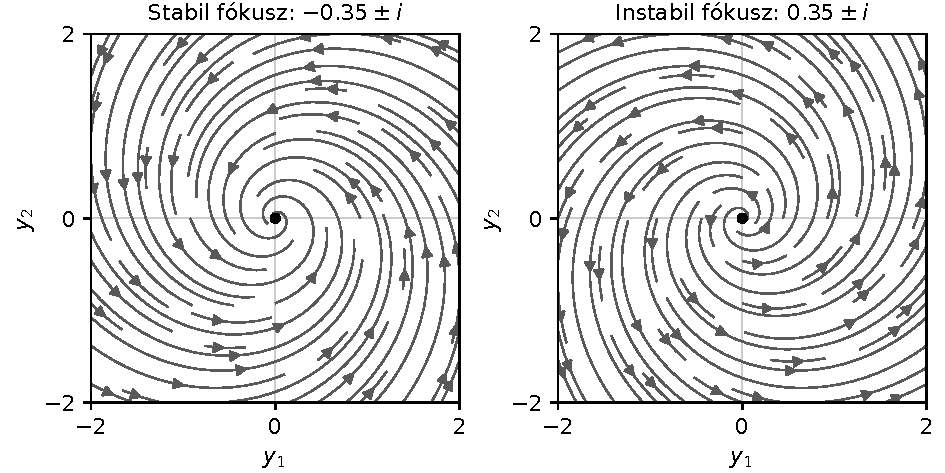
\includegraphics[width=\linewidth]{graphics_v3/phase_foci.pdf}
\caption{Fókuszok: $\lambda_{1,2}=-0{,}35\pm i$ (balra) és $\lambda_{1,2}=0{,}35\pm i$ (jobbra). A stabil fókusz pályái befelé, az instabiléi kifelé spiráloznak.}\label{fig:phase_foci}
\end{figure}

$\alpha=0$ esetén ebben a \emph{lineáris} rendszerben a sugár állandó: centrumot kapunk, amely stabil, de nem aszimptotikusan stabil. Egy nemlineáris rendszer tisztán képzetes sajátértékei azonban önmagukban nem garantálnak centrumot.

\paragraph*{Osztályozás nyom és determináns alapján.}
Valós $2\times2$ mátrixnál legyen $\tau=\operatorname{tr}A$, $\Delta=\det A$, $D=\tau^2-4\Delta$. A karakterisztikus egyenlet
\[
\lambda^2-\tau\lambda+\Delta=0
\]
alapján $\Delta<0$ nyerget, $\Delta>0$, $D>0$ csomópontot, $\Delta>0$, $D<0$, $\tau\neq0$ fókuszt jelent. Az utóbbi két eset stabil, ha $\tau<0$, és instabil, ha $\tau>0$. A $D=0$ ismétlődő, nemnulla sajátérték esetén a sajátvektorokat is vizsgáljuk: lehet csillagcsomó vagy egyetlen sajátirányú, degenerált csomó. $\Delta=0$ vagy $\tau=0$, $\Delta>0$ esetén nemhiperbolikus határesethez érünk.

A csomó és a fókusz geometriailag különbözik, de azonos stabilitás mellett topologikusan ekvivalens lehet. A topologikus ekvivalencia nem őrzi meg a szögeket, a görbületet vagy a spirálalakot. Hiperbolikus pontnál a nemlineáris és a linearizált rendszer lokális topologikus ekvivalenciáját a Hartman--Grobman-tétel biztosítja \cite[2.1.4. szakasz, 2.2. tétel]{dib}.

\FloatBarrier
\subsection{Az $N$ dimenziós rendszer linearizálása}
Legyen $x\in\mathbb R^N$, $f$ az $x^*$ környezetében legalább $C^1$, és $f(x^*)=0$. Vezessük be a $y=x-x^*$ eltérést. A Taylor-kifejtésből
\begin{equation}\label{eq:equilibrium_linearization_N}
\dot y=f(x^*+y)=Ay+R(y),\qquad
A=Df(x^*)=\left[\frac{\partial f_i}{\partial x_j}(x^*)\right]_{i,j=1}^{N},
\end{equation}
ahol $\|R(y)\|/\|y\|\to0$, ha $y\to0$. $f\in C^2$ esetén a maradék erősebb, $R(y)=O(\|y\|^2)$ becslést is kielégít. Az $A$ a \emph{Jacobi-mátrix}; a teljes linearizált vektormező $Ay$.

A maradéktagot elhagyva a konstans együtthatós
\begin{equation}\label{eq:linear_solution_N}
\dot y=Ay,\qquad y(t)=e^{At}y(0)
\end{equation}
rendszert kapjuk. Ez az egyensúly körüli közelítés, nem egy általános pálya körüli variációs egyenlet: ott a mátrix az időben változó referenciaállapot miatt $A(t)=Df(x(t))$. Az alapfelírást és a stabilitási kapcsolatot di Bernardo és szerzőtársai \cite[2.1.3--2.1.4. szakasz]{dib}, az általános hiperbolikus geometriát Kuznetsov \cite[2.2.1. szakasz]{kuznetsov_book} tárgyalja.

\subsection{Főtengelytranszformáció és modális koordináták}
\paragraph*{Diagonalizálható mátrix.}
Tegyük fel először, hogy $A$-nak van $N$ lineárisan független sajátvektora:
\[
Av_j=\lambda_jv_j,\qquad
S=[v_1\ \cdots\ v_N],\qquad
\Lambda=\operatorname{diag}(\lambda_1,\ldots,\lambda_N).
\]
Mivel $AS=S\Lambda$, a $y=Sz$ koordinátacsere után
\begin{equation}\label{eq:modal_transform}
S\dot z=ASz,\qquad
\dot z=S^{-1}ASz=\Lambda z.
\end{equation}
A modális egyenletek szétválnak:
\begin{equation}\label{eq:modal_solution}
\dot z_j=\lambda_jz_j,\qquad
z_j(t)=z_j(0)e^{\lambda_jt},\qquad
y(t)=\sum_{j=1}^{N}z_j(0)e^{\lambda_jt}v_j.
\end{equation}
Ez mutatja meg a sajátértékek szerepét: a sajátirányokhoz vagy invariáns síkokhoz tartozó amplitúdók növekedési ütemét adják. A báziscserét és a sajátértékeket Kuznetsov \cite[A.1.2--A.1.3. szakasz]{kuznetsov_book} foglalja össze.

A \emph{főtengelytranszformáció} elnevezést itt sajátvektor-bázisra való áttérésként használjuk. Általános, nem szimmetrikus Jacobi-mátrixnál $S$ nem feltétlenül ortogonális: a transzformáció nyírást és skálázást is tartalmazhat, és $S^{-1}\neq S^\mathsf T$. Valós szimmetrikus $A$ esetén választható ortonormált sajátvektor-bázis, ekkor valóban $S^{-1}=S^\mathsf T$. Egy általános dinamikai rendszerben a Jacobi-mátrix szimmetriáját nem tételezhetjük fel.

\exampleheading{Példa: nem merőleges sajátirányok.}
Legyen
\begin{equation}\label{eq:nonorthogonal_example}
A=\begin{pmatrix}-1&1\\0&-2\end{pmatrix},\qquad
S=\begin{pmatrix}1&-1\\0&1\end{pmatrix},\qquad
S^{-1}AS=\begin{pmatrix}-1&0\\0&-2\end{pmatrix}.
\end{equation}
A sajátvektorok $(1,0)^\mathsf T$ és $(-1,1)^\mathsf T$, amelyek nem merőlegesek. A $y=Sz$ átalakítás $y_1=z_1-z_2$, $y_2=z_2$, és az új egyenletek $\dot z_1=-z_1$, $\dot z_2=-2z_2$. A stabilitás nem változik a báziscserével, a pályák alakja viszont igen.
\exampleend

\paragraph*{Komplex sajátértékpár valós leírása.}
Valós $A$ esetén a nemvalós sajátértékek konjugált párokban jelennek meg. Ha $\lambda=\alpha+i\beta$ sajátvektora $v=p+iq$, akkor a $p,-q$ valós bázisban az adott invariáns sík mátrixa a \eqref{eq:focus_block} blokk. Így komplex koordináták használata nélkül is megkapjuk a forgást és az $e^{\alpha t}$ amplitúdóváltozást. A többi sajátirányhoz tartozó koordináták ettől függetlenül kezelhetők, ha az egész mátrix diagonalizálható a komplex számok felett.

\paragraph*{Ha nincs elegendő sajátvektor.}
Ismétlődő sajátérték nem feltétlenül jelent problémát, de előfordulhat, hogy $A$ nem diagonalizálható. Ilyenkor általánosított sajátvektorokkal Jordan-alakra térünk át, $S^{-1}AS=J$ \cite[A.1.4. szakasz, A.1. tétel]{kuznetsov_book}. Egy kétdimenziós Jordan-blokk például
\begin{equation}\label{eq:jordan_exponential}
J=\begin{pmatrix}\lambda&1\\0&\lambda\end{pmatrix},\qquad
e^{Jt}=e^{\lambda t}\begin{pmatrix}1&t\\0&1\end{pmatrix}.
\end{equation}
Nagyobb blokkoknál magasabb fokú időpolinomok is megjelennek. Ha $\operatorname{Re}\lambda<0$, az exponenciális lecsengés minden ilyen polinomot elnyom. Nulla valós résznél viszont a polinomiális tényező növekedést okozhat: a stabilitási határon a Jordan-szerkezetet is vizsgálni kell.

\subsection{Az egyensúly stabilitásának általános kritériuma}
\paragraph*{Mit értünk stabilitáson?}
Az $x^*$ egyensúly \emph{Ljapunov-stabil}, ha minden elegendően kis $\varepsilon>0$ számhoz található $\delta>0$, hogy
\begin{equation}\label{eq:lyapunov_stability_definition}
\|x(0)-x^*\|<\delta
\quad\Longrightarrow\quad
\|x(t)-x^*\|<\varepsilon\quad\text{minden }t\geq0\text{ esetén}.
\end{equation}
\emph{Lokálisan aszimptotikusan stabil}, ha emellett egy környezetéből induló minden megoldás $x^*$-hoz tart. \emph{Lokálisan exponenciálisan stabil}, ha valamely $C,\gamma>0$ mellett, elég kis kezdeti eltérésekre
\begin{equation}\label{eq:exponential_stability}
\|x(t)-x^*\|\leq Ce^{-\gamma t}\|x(0)-x^*\|.
\end{equation}
Az aszimptotikus stabilitás tehát többet állít a közelség megőrzésénél. A definíciókat lásd \cite[2.1.3. szakasz, 2.9--2.10. definíció]{dib} és \cite[1.3.3. szakasz]{kuznetsov_book}.

\paragraph*{Lineáris rendszer: teljes spektrális feltétel.}
A $\dot y=Ay$ origója pontosan akkor aszimptotikusan stabil, ha
\begin{equation}\label{eq:hurwitz_criterion}
\boxed{\operatorname{Re}\lambda_j(A)<0\qquad(j=1,\ldots,N).}
\end{equation}
Ekkor exponenciálisan is stabil; az ilyen mátrixot Hurwitz-mátrixnak nevezzük. A feltétel a nem diagonalizálható mátrixokra is igaz. A megoldás normája közben átmenetileg nőhet, különösen nem merőleges sajátirányok mellett; az exponenciális becslés $C$ szorzója ezért nem feltétlenül egy. Ha valamely sajátérték valós része pozitív, az origó instabil.

A lineáris rendszer \emph{Ljapunov-stabilitásának} szükséges és elégséges feltétele az, hogy minden sajátértékre $\operatorname{Re}\lambda_j\leq0$, és a képzetes tengelyen fekvő sajátértékekhez csak egydimenziós komplex Jordan-blokkok tartozzanak. Utóbbit semisimple sajátértéknek is mondjuk. Ilyen centrumirányok jelenlétében a megoldás korlátos maradhat, de általában nem tart az origóhoz. A $J=\left(\begin{smallmatrix}0&1\\0&0\end{smallmatrix}\right)$ ellenpélda: minden sajátértéke nulla, mégis $y_1(t)=y_1(0)+t\,y_2(0)$, ezért instabil.

\paragraph*{Nemlineáris rendszer: a linearizálás hatóköre.}
Az $f\in C^1$ rendszer $x^*$ egyensúlyánál, $A=Df(x^*)$ jelöléssel:
\begin{itemize}
\item Ha minden sajátérték valós része negatív, $x^*$ lokálisan exponenciálisan, így aszimptotikusan stabil.
\item Ha legalább egy sajátérték valós része pozitív, $x^*$ instabil, akkor is, ha más sajátértékek valós része nulla.
\item Ha nincs pozitív valós rész, de van nulla valós részű sajátérték, a linearizálás általában nem dönt a nemlineáris stabilitásról.
\end{itemize}
Az utolsó esetben nem szabad a lineáris centrum stabilitását automatikusan átvinni a nemlineáris rendszerre. Például a $\dot x=-x^3$ és a $\dot x=x^3$ egyenlet origójában ugyanaz az $A=0$ linearizálás, de az első egyensúly aszimptotikusan stabil, a második instabil. A negatív valós részű spektrum ezért elégséges, de nem szükséges feltétele a nemlineáris aszimptotikus stabilitásnak. A nemhiperbolikus esetekhez magasabb rendű tagok, középponti sokaság vagy Ljapunov-függvény vizsgálata szükséges; lásd \cite[5.1--5.2. szakasz]{kuznetsov_book}.

Ha egyik sajátérték valós része sem nulla, az egyensúly \emph{hiperbolikus}. A negatív és pozitív valós részű sajátértékek algebrai multiplicitással számított száma $N_s$, illetve $N_u$, és $N_s+N_u=N$. A lokális stabil és instabil sokaság dimenziója rendre $N_s$, illetve $N_u$; az egyensúlyban a megfelelő általánosított sajátalterek érintik őket. $N_s>0$, $N_u>0$ esetén $N$ dimenzióban is nyeregpontot kapunk \cite[2.2.1. szakasz, 2.1. tétel]{kuznetsov_book}.

\paragraph*{Ljapunov-függvény és a mátrixfeltétel kapcsolata.}
A spektrális eredmény energiaszerű becsléssel is értelmezhető. Hurwitz-mátrixhoz minden $Q=Q^\mathsf T>0$ mellett létezik egyértelmű $P=P^\mathsf T>0$, amelyre
\begin{equation}\label{eq:lyapunov_matrix}
A^\mathsf TP+PA=-Q.
\end{equation}
Ekkor $V(y)=y^\mathsf TPy$ pozitív definit, és a lineáris rendszerben $\dot V=-y^\mathsf TQy<0$ minden $y\neq0$ esetén. A nemlineáris rendszerben
\[
\dot V=-y^\mathsf TQy+2y^\mathsf TPR(y),
\]
és a maradék $o(\|y\|^2)$, ezért elegendően kis környezetben a negatív kvadratikus tag dominál. Ez a lokális stabilitást igazolja; a vonzási tartomány teljes méretét nem határozza meg.

Általánosabban, egy $C^1$, pozitív definit $V$ függvény és a pálya menti negatív definit $\dot V$ lokális aszimptotikus stabilitást biztosít; $\dot V\leq0$ önmagában rendszerint csak stabilitást igazol. A $\dot x=-x^3$ példában $V=x^2/2$, $\dot V=-x^4$, így a módszer a nulla sajátérték ellenére dönt. A szemléletet di Bernardo és szerzőtársai \cite[2.1.3. és 2.4.1. szakasz]{dib} kapcsolja a szakaszos rendszerek stabilitásvizsgálatához.

Végül a fenti Jacobi-kritérium \emph{sima környezetben fekvő} egyensúlyra vonatkozik. Kapcsolófelületen elhelyezkedő pontnál a két oldali mátrix külön vizsgálata általában nem elegendő; a sliding dinamikát, az átmeneti szabályokat vagy a boundary equilibrium geometriáját is figyelembe kell venni \cite[2.4.1. szakasz és 5. fejezet]{dib}.

\section{Stabilitásvesztési formák}
Az egyensúlyok sima bifurkációinak könyvbeli háttere: \cite[2.1.6. szakasz]{dib} és \cite[3.1--3.5. szakasz]{kuznetsov_book}.

A Hopf-bifurkáció részletes feltételeit \cite{kuznetsov} foglalja össze.

Sima, egyparaméteres síkbeli rendszerek egyensúlyainak generikus lokális bifurkációi közül két alapvető eset a saddle-node bifurcation és a Hopf-bifurkáció. Saddle-node bifurcation esetén egy egyszerű sajátérték nullává válik, és megfelelő nemelfajulási feltételek mellett két egyensúlyi ág találkozik és megszűnik, illetve keletkezik. Hopf-bifurkációnál egy komplex konjugált sajátértékpár $\lambda_{1,2}(\mu)=\alpha(\mu)\pm i\omega(\mu)$ halad át a képzetes tengelyen: $\alpha(\mu_0)=0$, $\omega(\mu_0)>0$ és $\alpha'(\mu_0)\neq0$. A generikus esethez az első Ljapunov-együttható nemnullasága is szükséges.

Szuperkritikus Hopf-bifurkációnál stabil, kis amplitúdójú határciklus születik; szubkritikus esetben a lokálisan megjelenő határciklus instabil. Az utóbbi esetben fellépő véges amplitúdójú ugrás és hiszterézis a további, globális dinamikától függ. Szimmetriák vagy más speciális feltételek mellett transcritical bifurcation és pitchfork bifurcation is előfordulhat.

\section{Periodikus pályák, monodrómia-mátrix}
A Poincaré-leképezéshez és a periodikus pálya stabilitásához lásd \cite[2.1.5. szakasz]{dib}, illetve \cite[1.5. és 2.2.3. szakasz]{kuznetsov_book}.


Tekintsük az $\dot{x}=f(x)$ dinamikai rendszer $x(t)=p(t)$ $T$ periódusú periodikus pályáját, azaz $p(t)=p(t+T)$. A pálya közelében szeretnénk a dinamikát vizsgálni, ezért megkonstruáljuk az ún. \emph{Poincaré-metszetet}, amely egy $n-1$ dimenziós $\Pi$ felület, amely tartalmazza az $x_p=p(t^*)$ pontot és transzverzálisan metszi a pályát (= nem érinti).

Legyen a Poincaré-metszetet definiáló felület: $\Pi = \{x\in\mathbb{R}^n:\pi(x)=0\}$! Ekkor a transzverzalitás feltétele, hogy Poincaré felületre merőleges vektornak ($\pi_x$) $x_p$-ben legyen a trajektória irányába eső vetülete, azaz $\pi_x(x_p) f(x_p)=<\pi_x(x_p), f(x_p)>\neq 0$.

A Poincaré leképezés ezek után, ha $x$ megfelelően közel van $x_p$-hez, a $P(x)=\Phi(x,\tau(x))$ alakban írható, ahol $\tau(x)$-et (a megzavart pálya visszatérési idejét) a $\pi(\Phi(x,\tau(x)))=0$ egyenlet definiálja. Itt $\tau(x)$ visszatérési idő; egy közeli, nemperiodikus pályának általában nincs periódusa.

A periodikus pálya stabilitását az ún. \emph{monodrómia-mátrix} kiszámításával lehet vizsgálni. Vizsgáljuk a
\begin{equation}
\dot{x}=A(t)x
\label{eq:per_lin}
\end{equation}
dinamikai rendszert, melyben $A(t)$ periodikus $T$ periódussal. Legyen $X(t)$ \eqref{eq:per_lin} fundamentális megoldásmátrixa, azaz $n$ darab lineárisan független megoldásból képzett mátrix. Ekkor létezik olyan \emph{konstans} $C$ mátrix, melyre $X(t+T)=X(t)C$. Továbbá, ennek kiszámítása egyszerű, hiszen $t=0$-ban $X(T)=X(0)C$, tehát $C=X^{-1}(0)X(T)$. Továbbá, ha $X(0)=I$, akkor $C=X(T)$. A $C$ mátrix a monodrómia reprezentációja az $X(0)$ bázisban; az állapotkoordinátákban a mátrix $X(T)X(0)^{-1}$. A két mátrix hasonló, ezért multiplikátoraik azonosak.

Így az eredeti $\dot{x}=f(x)$ dinamikai rendszer $p(t)$ periodikus pályája körül linearizálva kapjuk az $\dot y =f'(p(t))y$ variációs egyenletet, melynek a \emph{fundamentális megoldását} kell $t=T$ pillanatban kiszámítani, ahol $T$ a periódusidő. Ezt legegyszerűbben úgy tehetjük meg, ha speciális kezdeti feltételekből numerikusan integráljuk az egyenletet:
\[
\mathbf{M}=\begin{bmatrix}
\Phi_p(\mathbf{e}_1,T) & \cdots & \Phi_p(\mathbf{e}_n,T)
\end{bmatrix}
\]
ahol $\Phi_p$ a variáció egyenlet fundamentális megoldás operátora, $\mathbf{e}_i$ az i-edik egységvektor. Nemállandó autonóm periodikus pálya esetén az időeltolási irányhoz $1$ multiplikátor tartozik. Ha ez egyszeres, és minden további multiplikátorra $|\lambda_j|<1$, a pálya orbitálisan aszimptotikusan stabil. Ha valamelyikre $|\lambda_j|>1$, a pálya instabil; további egységkörön fekvő multiplikátorok esetén a linearizálás általában nem dönt. A Poincaré-leképezés deriváltja a transzverzális, nemtriviális multiplikátorokat tartalmazza.

A fundamentális megoldásmátrixot most $\Phi(t)$ jelöli; ekkor $\Phi(t+T)=\Phi(t)B$. A konstans $B\in\mathbb R^{n\times n}$ mátrix pontos definíciója a $t=0$ helyettesítésből:
\[
\Phi(T)=\Phi(0)B,\qquad
\boxed{B=\Phi(0)^{-1}\Phi(T)}.
\]
Ez az előbb $C$-vel jelölt mátrix, a választott fundamentális megoldás kezdőbázisában. Ha $\Phi(0)=I$, akkor
\[
B=\Phi(T)=\begin{bmatrix}y_1(T)&\cdots&y_n(T)\end{bmatrix}=\mathbf M,
\qquad \dot y_j=A(t)y_j,\quad y_j(0)=e_j.
\]
Tehát oszlopai az egységvektorokból indított variációs megoldások egy periódus utáni értékei. Általános kezdőbázisnál az állapotkoordinátákban vett monodrómia-mátrix $\mathbf M=\Phi(T)\Phi(0)^{-1}=\Phi(0)B\Phi(0)^{-1}$; normalizált kezdőbázisnál $B=\mathbf M$. A determinánst Liouville formulája adja:


\begin{equation}
\det(B)=\exp \left( \int_0^T \mathrm{tr}(A(s)) ds\right).
\end{equation}

\exampleheading{Példa: a fundamentális megoldásmátrix előállítása.}
Először egy egyszerű, csatolt lineáris rendszeren végezzük el az oszloponkénti konstrukciót. Dimenziótlan idővel és állapotokkal legyen
\begin{equation}\label{eq:fundamental_example_system}
 \dot y=Ay,\qquad
 A=\begin{pmatrix}-1&1\\0&-2\end{pmatrix},\qquad
 \begin{cases}\dot y_1=-y_1+y_2,\\\dot y_2=-2y_2.\end{cases}
\end{equation}
Ez két lecsengő folyamat egyszerű modellje: a második állapot gerjeszti az elsőt, visszahatás azonban nincs. A normalizált fundamentális megoldásmátrixot $X(t)$ jelöli; azt keressük, amelyre
\begin{equation}\label{eq:fundamental_example_ivp}
 \dot X(t)=AX(t),\qquad X(0)=I.
\end{equation}
A mátrix minden oszlopa ugyanannak a differenciálegyenletnek egy megoldása, de más kezdeti állapotból indul. Az oszlopokat $y^{(1)}$ és $y^{(2)}$ jelöli; a zárójeles felső index itt a megoldást sorszámozza, nem deriválást jelent.

Az első oszlophoz $y^{(1)}(0)=e_1=(1,0)^{\mathsf T}$ kezdeti állapotot választunk.
A második egyenletből $y_2^{(1)}(t)=0$. Ezt az elsőbe helyettesítve $\dot y_1^{(1)}=-y_1^{(1)}$, $y_1^{(1)}(0)=1$, tehát
\[
 y^{(1)}(t)=\begin{pmatrix}e^{-t}\\0\end{pmatrix}.
\]
A második oszlophoz $y^{(2)}(0)=e_2=(0,1)^{\mathsf T}$ kezdeti állapot tartozik.
Most $y_2^{(2)}(t)=e^{-2t}$. Az első komponens egyenlete és kezdeti feltétele
\[
 \dot y_1^{(2)}+y_1^{(2)}=e^{-2t},\qquad y_1^{(2)}(0)=0.
\]
Az $e^t$ integráló tényezővel szorozva, majd $0$ és $t$ között integrálva
\[
 \frac{d}{dt}\bigl(e^t y_1^{(2)}(t)\bigr)=e^{-t},\qquad
 e^t y_1^{(2)}(t)=\int_0^t e^{-s}\,ds=1-e^{-t}.
\]
Így $y_1^{(2)}(t)=e^{-t}-e^{-2t}$, és
\[
 y^{(2)}(t)=\begin{pmatrix}e^{-t}-e^{-2t}\\e^{-2t}\end{pmatrix}.
\]

\begin{equation}\label{eq:fundamental_example_matrix}
 \boxed{X(t)=\begin{bmatrix}y^{(1)}(t)&y^{(2)}(t)\end{bmatrix}
 =\begin{pmatrix}e^{-t}&e^{-t}-e^{-2t}\\0&e^{-2t}\end{pmatrix}.}
\end{equation}
Közvetlenül látható, hogy $X(0)=I$. A differenciálegyenlet ellenőrzése is egyszerű:
\[
 \dot X(t)=\begin{pmatrix}-e^{-t}&-e^{-t}+2e^{-2t}\\0&-2e^{-2t}\end{pmatrix}
 =AX(t).
\]
Továbbá $\det X(t)=e^{-3t}\neq0$ minden véges $t$ esetén, ezért az oszlopok lineárisan függetlenek: valóban fundamentális megoldásmátrixot kaptunk. A determináns megegyezik a Liouville-formula eredményével, hiszen $\operatorname{tr}A=-3$.


Ha $y(0)=(a,b)^{\mathsf T}$, a linearitás miatt
\begin{equation}\label{eq:fundamental_example_solution}
 y(t)=X(t)y(0)=a\,y^{(1)}(t)+b\,y^{(2)}(t)
 =\begin{pmatrix}a e^{-t}+b(e^{-t}-e^{-2t})\\b e^{-2t}\end{pmatrix}.
\end{equation}
Az $X_{12}(t)$ elem tehát azt mutatja meg, hogyan hat a második állapot kezdeti eltérése az első állapot későbbi értékére. A kezdeti egységmátrix oszlopai nem maradnak állandók: mindegyiket a dinamika szerint továbbvezetjük. Mivel itt $A$ állandó, $X(t)=e^{At}$ is írható; a fenti számítás ezt a mátrixexponenciálist állította elő.


A konstans $A$ bármely $T>0$ választással periodikus együtthatómátrixnak tekinthető. Egy ilyen rögzített időszakaszra $\mathbf M=X(T)$, sajátértékei $e^{-T}$ és $e^{-2T}$. Ebben a példában azonban egy stabil egyensúly körüli rendszert vizsgálunk, nem egy nemállandó autonóm periodikus pálya variációs egyenletét. Ezért nincs kötelező, időeltoláshoz tartozó egységnyi multiplikátor. A következő példa már egy határciklushoz tartozó fundamentális megoldásmátrixot és monodrómia-mátrixot mutat be.
\exampleend

\exampleheading{Példa: határciklus fundamentális megoldásmátrixa.} Tekintsük a következő rendszert: $\dot{r}=r (1-r^2)$ és $\dot{\phi} = 1$. A határciklus polárkoordinátákban $r(t)=1$, $\phi(t)=t$ (modulo $2\pi$), vagyis az $(x,y)$ koordináta-rendszerben $p(t) = \{(x,y)=(\cos t,\sin t):t\in\mathbb{R}\}$.

A radiális perturbáció legyen $\rho=r-1$. Linearizálva $\dot{\rho}=-2\rho$, ezért a radiális eltérések lecsengenek. A fázisirány semleges; a stabilitás orbitális értelemben értendő.

A pálya vizsgálatához térjünk át derékszögű koordináta rendszerre!

\begin{align}
x=r\cos \phi& \quad \rightarrow \quad & \dot{x}=\dot{r} \cos \phi-r \sin\phi\, \dot{\phi}=x\left(1-x^2-y^2\right)-y\\
y=r\sin \phi& \quad \rightarrow \quad & \dot{y}=\dot{r} \sin \phi+r \cos\phi\, \dot{\phi}=y\left(1-x^2-y^2\right)+x
\end{align}

Itt kihasználtuk, hogy pl. $\dot{r}\cos \phi=r\cos\phi(1-r^2)=x(1-(x^2+y^2))$ ill. $\dot{\phi}=1$. A fenti dinamikai rendszer  általános linearizáltja és annak periodikus pálya közelében vett alakja:
\begin{equation}
f'(p(t)) = \left. \begin{pmatrix}
1-3x^2-y^2 & -1-2xy \\
1-2xy & 1-x^2-3y^2 \\
\end{pmatrix} \right|_{p(t)}=
\begin{pmatrix}
-2\cos^2t & -1-\sin 2t \\
1-\sin 2t & -2\sin^2t \\
\end{pmatrix}
\end{equation}

Így a perturbációs egyenlet

\begin{equation}
\dot{z}=\begin{pmatrix}
-2\cos^2t & -1-\sin 2t \\
1-\sin 2t & -2\sin^2t \\
\end{pmatrix} z
\end{equation}

A monodrómia-mátrix determinánsát analitikusan is ki tudjuk számítani:

\begin{align}
\det(B)&=\exp \left( \int_0^T \mathrm{tr}(A(t)) dt\right)=\exp \left( \int_0^T -2\cos^2t-2\sin^2t dt\right)\\
&=\exp \left( \int_0^T -2 dt\right)=e^{-4\pi}<1.
\end{align}

A determináns természetesen a sajátértékek (karakterisztikus multiplikátorok) szorzata, ám (periodikus pályáról lévén szó) az egyik sajátérték biztosan 1, mivel pedig itt kétdimenziós rendszerről van szó, a második pontosan a fenti eredmény. A $p(0)=(1,0)$ kezdőpontnál a monodrómia-mátrix pontos alakja (amelyet a numerikus integrálás közelít):

\begin{equation}
\mathbf{M}=\begin{pmatrix}
e^{-4\pi} & 0\\ 0 & 1\\
\end{pmatrix}.
\end{equation}

Mivel $e^{-4\pi}<1$, $p(t)$ pálya orbitálisan aszimptotikusan stabil. A függelékben közölt MATLAB-kód a variációs egyenletet integrálja, és a kapott mátrixot a pontos $\operatorname{diag}(e^{-4\pi},1)$ mátrixszal ellenőrzi. Az egységnyi multiplikátort a numerikus hiba erejéig kell visszakapnunk.

\phantomsection\label{use:monodromy}A teljes MATLAB-program az A függelék \ref{ap:monodromy}. szakaszában található (\pageref{ap:monodromy}. oldal).
\exampleend

\exampleheading{Példa: periodikus együtthatómátrix.\footnote{E. Folkers: Floquet’s Theorem, Bachelor’s Project Mathematics, University of Groningen}} Tekintsük a következő rendszert:
\begin{equation}
\dot{x}=A(t)x=\begin{pmatrix}
-1 & 1\\
0 & 1+ \cos t-\frac{\sin t}{2+\cos t}
\end{pmatrix}x.
\end{equation}

(Ebben az esetben \emph{nem} egy autonóm rendszer periodikus pályája körüli linearizált rendszert vizsgálunk, hanem egy általános lineáris rendszert periodikus együtthatómátrixszal: $A(t)=A(t+2\pi)$.) A rendszer megoldása:
\begin{align}
x_1(t)&=c_2 e^{t+\sin t}+c_3 e^{-t}\\
x_2(t)&=c_2e^{t+\sin t}\left( 2+\cos t\right).
\end{align}

A két független megoldást oszlopokba rendezve egy fundamentális mátrix:
\begin{equation}
X(t)=
\begin{pmatrix}
e^{t+\sin t} &  e^{-t}\\
e^{t+\sin t}\left( 2+\cos t\right) &0
\end{pmatrix},
\end{equation}

mivel az általános megoldás $x(t)=c_2 X_1(t)+c_3 X_2(t)$ alakban írható, ahol $X_i$ a fundamentális mátrix $i$-edik oszlopát jelenti. A monodrómia-mátrix:
\begin{align}
C&=X^{-1}(0)X(2\pi)\\
&=\begin{pmatrix}0&1/3\\1&-1/3\end{pmatrix}
\begin{pmatrix}e^{2\pi}&e^{-2\pi}\\3e^{2\pi}&0\end{pmatrix}
=\begin{pmatrix}e^{2\pi}&0\\0&e^{-2\pi}\end{pmatrix}.
\end{align}
A multiplikátorok $\lambda_1=e^{2\pi}\approx535{,}492$ és $\lambda_2=e^{-2\pi}\approx0{,}00186744$, ezért a zérusmegoldás instabil. Itt általános periodikus lineáris rendszerről van szó, így nem szükséges, hogy legyen egységnyi multiplikátor.
\exampleend

\section{Bifurkációk}

\subsection{Egyensúlyi helyzetek bifurkációi}\label{sec:eq_bif_types}
Az alábbi lista sima, egyparaméteres rendszerek helyi bifurkációit foglalja össze. Legyen $A=f_x(x^*,\mu)$, a kritikus paraméter az átskálázás után $\mu=0$. A megadott egyszerű normálalakok a kritikus irányok dinamikáját szemléltetik; az ábrák stabilitásjelöléseihez a többi sajátérték valós részét negatívnak feltételezzük. A kritikus sajátértékfeltétel önmagában nem elegendő: a paraméterfüggés és a vezető nemlineáris tag sem lehet elfajuló. Háttér: \cite[2.1.6. szakasz]{dib}, \cite[3. fejezet]{kuznetsov_book}.
\begin{itemize}
\item \textbf{Saddle-node bifurcation.} Egy stabil és egy instabil egyensúly találkozik és eltűnik, illetve keletkezik. \textit{Feltétel:} egy egyszerű $\lambda=0$ sajátérték; a redukált $\dot u=g(u,\mu)$ egyenletben $g_\mu\neq0$, $g_{uu}\neq0$. Példa: $\dot u=\mu-u^2$; $\mu>0$ esetén $u^*=\pm\sqrt\mu$.
\item \textbf{Transcritical bifurcation.} Két fennmaradó egyensúlyi ág keresztezi egymást és stabilitást cserél. \textit{Feltétel:} egyszerű $\lambda=0$, továbbá a két ág fennmaradását biztosító struktúra. Az egyik ágat $u=0$-ra helyezve $g(0,\mu)=0$, $g_{u\mu}\neq0$, $g_{uu}\neq0$. Példa: $\dot u=\mu u-u^2$, ágai $u^*=0$ és $u^*=\mu$.
\item \textbf{Pitchfork bifurcation.} Egy egyensúlyi ágból két szimmetrikus ág válik ki. \textit{Feltétel:} egyszerű $\lambda=0$, az $u\mapsto-u$ szimmetriát biztosító struktúra, $g_{u\mu}\neq0$, $g_{uuu}\neq0$. \textit{Supercritical} esetben $\dot u=\mu u-u^3$: $\mu>0$ mellett két stabil ág születik. \textit{Subcritical} esetben $\dot u=\mu u+u^3$: $\mu<0$ mellett két instabil mellékág van.
\item \textbf{Hopf-bifurkáció.} Az egyensúly körül kis amplitúdójú periodikus pálya jelenik meg vagy tűnik el. \textit{Feltétel:} egy egyszerű $\lambda_{1,2}=\pm i\omega_0$ pár, $\omega_0>0$, $d\operatorname{Re}\lambda/d\mu\neq0$, és nemnulla első Ljapunov-együttható. A $\dot r=\mu r-r^3$, $\dot\theta=\omega_0$ normálalak \textit{supercritical}: a stabil ciklus amplitúdója $r=\sqrt\mu$. A $\dot r=\mu r+r^3$ \textit{subcritical}: az instabil ciklus $r=\sqrt{-\mu}$, $\mu<0$. A negatív $r$ értékek nem fizikai amplitúdók.
\end{itemize}
A transcritical és a pitchfork bifurcation általában nem marad fenn tetszőleges, a struktúrát megsértő perturbáció mellett. A Hopf-bifurkációt az egyensúly bifurkációi közé soroljuk, mert a kritikus objektum az egyensúly, még ha a megjelenő objektum periodikus pálya is.
\begin{figure}[!htbp]\centering
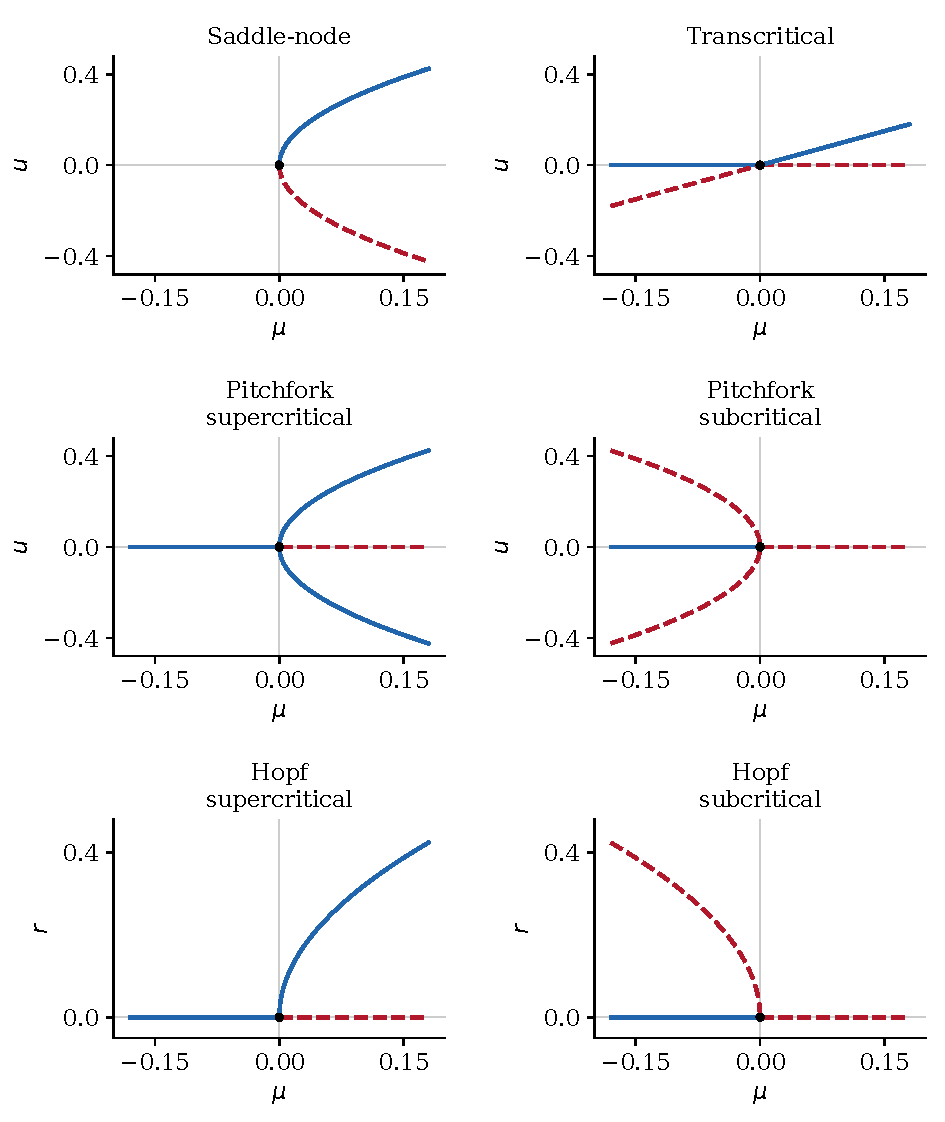
\includegraphics{graphics_v3/equilibrium_bifurcations.pdf}
\caption{Egyensúlyi bifurkációk normálalakjainak ágdiagramjai. Kék folytonos: stabil; piros szaggatott: instabil ág. Az első négy panelen $u^*$ egyensúlyi koordináta, az utolsó kettőn $r$ amplitúdó szerepel: ott $r=0$ az egyensúly, $r>0$ periodikus pálya. A fekete pont a kritikus állapot.}\label{fig:eq_bif_types}
\end{figure}
\FloatBarrier

\subsection{Periodikus pályák bifurkációi}\label{sec:cycle_bif_types}
Egy periodikus pályát a Poincaré-leképezés fixpontjaként vizsgálunk. Az alábbi $\rho$ értékek a transzverzális Floquet-multiplikátorok, vagyis $D P$ sajátértékei. Autonóm rendszerben a pálya menti időeltolás triviális $+1$ multiplikátorát előbb elhagyjuk. A többi, nemkritikus multiplikátor az ábrákon az egységkör belsejében van. Egy $m$ ciklusnál $D(P^m)$ vizsgálandó. Háttér: \cite[2.1.5--2.1.6. szakasz]{dib}, \cite[4--5. fejezet]{kuznetsov_book}.
\begin{itemize}
\item \textbf{Fold of cycles (saddle-node bifurcation of cycles).} Egy stabil és egy instabil periodikus pálya találkozik és eltűnik. \textit{Feltétel:} egyszerű, nemtriviális $\rho=+1$. A redukált leképezés $G(u,\mu)=P(u,\mu)-u$ maradékára $G_\mu\neq0$, $G_{uu}\neq0$. Szemléltető alak: $P(u,\mu)=u+\mu-u^2$.
\item \textbf{Period-doubling bifurcation.} A $T$ periódusú pálya stabilitást veszít, és egy hozzá közeli, közel $2T$ periódusú pálya jelenik meg. \textit{Feltétel:} egyszerű $\rho=-1$, $d\rho/d\mu\neq0$, és nemnulla redukált köbös együttható. A $P(u,\mu)=-(1+\mu)u+u^3$ \textit{supercritical} példa: a stabil kétciklus pontjai $u=\pm\sqrt\mu$. A köbös tag negatív előjelével a \textit{subcritical} esetben instabil kétciklus van $\mu<0$ mellett. Az ábra ugyanannak a megkettőzött pályának két metszéspontját mutatja.
\item \textbf{Neimark--Sacker-bifurkáció (torus bifurcation).} A Poincaré-leképezésben invariáns zárt görbe, a folytonos rendszerben invariáns tórusz jelenik meg a ciklus körül. \textit{Feltétel:} egyszerű $\rho_{1,2}=e^{\pm i\theta_0}$ pár, $d|\rho|/d\mu\neq0$, nemnulla első Ljapunov-együttható és $e^{ik\theta_0}\neq1$ ($k=1,2,3,4$). A radiális normálalak $r_{n+1}=(1+\mu)r_n-r_n^3$ \textit{supercritical}; a pozitív köbös tag \textit{subcritical} esetet ad. A tóruszon a mozgás nemrezonáns esetben kváziperiodikus, rezonanciánál periodikus mozgás is lehetséges. Autonóm folytonos rendszerben ehhez legalább három állapotváltozó kell.
\item \textbf{Transcritical bifurcation of cycles.} Két periodikus pálya ága keresztezi egymást és stabilitást cserél. \textit{Feltétel:} egyszerű, nemtriviális $\rho=+1$, a két ág fennmaradását biztosító struktúra; $G(0,\mu)=0$, $G_{u\mu}\neq0$, $G_{uu}\neq0$. Példa: $P(u,\mu)=u+\mu u-u^2$.
\item \textbf{Pitchfork bifurcation of cycles.} Egy szimmetrikus ciklusból két, egymás szimmetrikus képét adó ciklus válik ki. \textit{Feltétel:} egyszerű, nemtriviális $\rho=+1$, megfelelő szimmetria, $G_{u\mu}\neq0$, $G_{uuu}\neq0$. A $P(u,\mu)=u+\mu u-u^3$ \textit{supercritical}; pozitív köbös taggal \textit{subcritical}. A két mellékág itt két külön periodikus pálya, nem ugyanannak a kétciklusnak két pontja.
\end{itemize}
A normálalakok és stabilitásjelölések a kritikus pont kis környezetére vonatkoznak. A lista a sima helyi bifurkációkat foglalja össze; a globális homoclinic és heteroclinic eseményekre nincs önmagában elegendő helyi multiplikátorfeltétel. A piecewise-smooth rendszerek grazing, border-collision és sliding eseteit a későbbi fejezetek tárgyalják.
\begin{figure}[!htbp]\centering
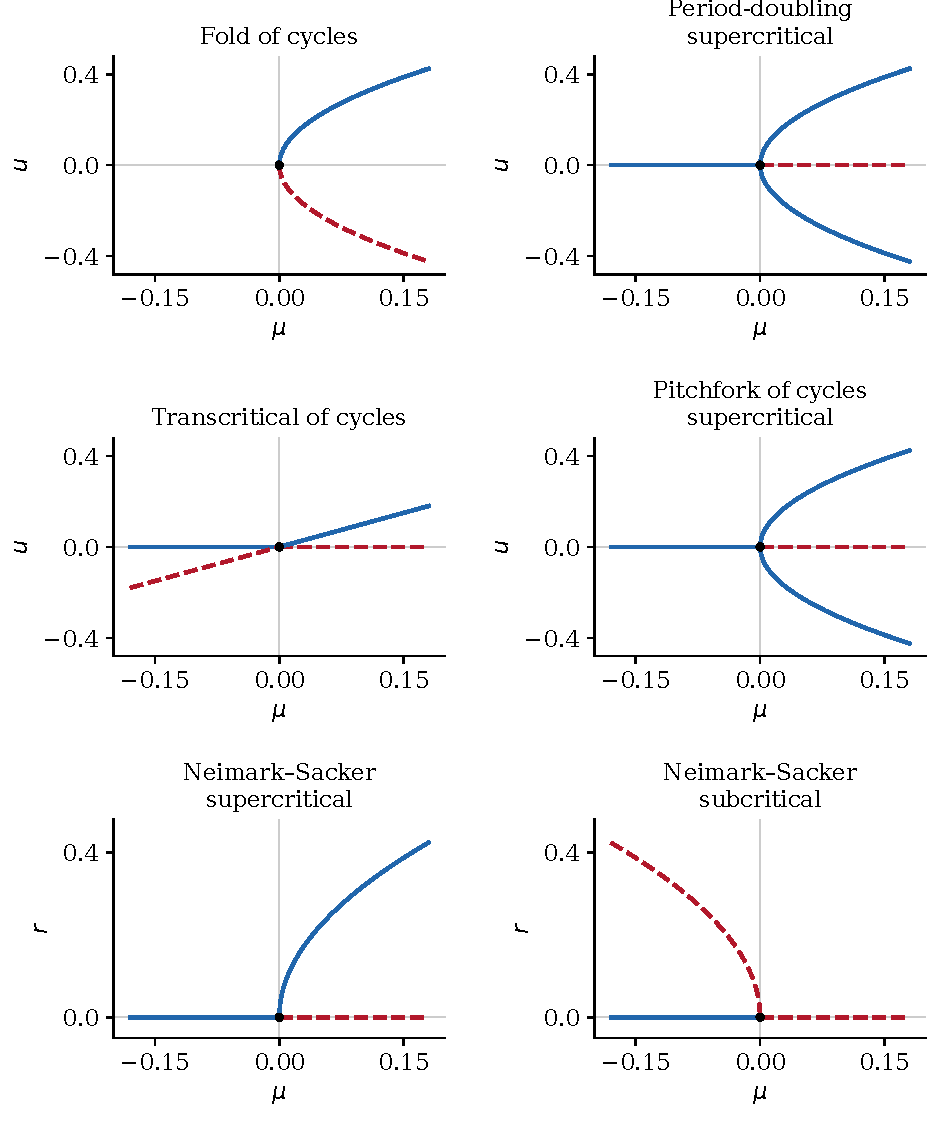
\includegraphics{graphics_v3/cycle_bifurcations.pdf}
\caption{Periodikus pályák helyi bifurkációi a Poincaré-metszeten. Kék folytonos: stabil; piros szaggatott: instabil. Az $u$ tengely a referenciaciklustól mért metszeti koordináta, nem a fizikai rezgésamplitúdó. A period-doubling panel két mellékága ugyanazon pálya két pontja, a pitchfork panel két mellékága két külön ciklus. A Neimark--Sacker-paneleken $r=0$ a kiinduló ciklus, $r>0$ az invariáns görbe sugara. A normálalakok helyi ágait ábrázoljuk.}\label{fig:cycle_bif_types}
\end{figure}
\FloatBarrier

\subsection{Szakadások osztályozása}\label{sec:discontinuity_types}
A szakaszos modelleknél először azt kell tisztázni, \emph{melyik mennyiség} folytonosságát vizsgáljuk: az erőt, a vektormezőt, annak deriváltját vagy magát az állapotot. Ezek eltérő tulajdonságok. Egy relé kapcsolásakor például az erő ugrik, miközben véges tömeg esetén a helyzet és a sebesség folytonos maradhat. Egy ideális merev ütközésnél viszont a sebesség ugrik.

Legyen $f$ egy $x_0$ környezetében, esetleg az $x_0$ pont kivételével értelmezett skalárfüggvény. Jelölje
\[
L_-=\lim_{x\to x_0^-}f(x),\qquad L_+=\lim_{x\to x_0^+}f(x)
\]
a két egyoldali határértéket. Folytonossághoz mindkettőnek léteznie kell, végesnek és egyenlőnek kell lenniük, továbbá $f(x_0)=L_-=L_+$ szükséges. Ha $f(x_0)$ nincs megadva, folytonos kiterjeszthetőségről beszélünk. Az alábbi osztályozásban az elsőfajú esetekhez mindkét véges egyoldali határérték létezését megköveteljük; minden más szakadást másodfajúnak nevezünk.

\paragraph{1. Megszüntethető szakadás: egy hibás vagy hiányzó pontérték.}
Ha $L_-=L_+=L\in\mathbb R$, de a pontérték hiányzik vagy $f(x_0)\neq L$, akkor az $f(x_0):=L$ hozzárendelés folytonossá teszi a függvényt. A görbe két oldala tehát illeszkedik; csak egy pontot kell helyesen kitölteni.

\exampleheading{Mérnöki példa: mozgóátlagoló szűrő zérus frekvencián.} Egy $\tau>0$ hosszúságú, középre igazított időablakon átlagoló szűrő frekvenciaválasza
\[
G(\omega)=\frac{\sin(\omega\tau/2)}{\omega\tau/2},\qquad \omega\neq0.
\]
A közvetlen képlet $\omega=0$-nál $0/0$ alakú, de a $\sin z=z+\mathcal O(z^3)$ sorfejtésből
\[
\lim_{\omega\to0}G(\omega)=1.
\]
A helyes kiterjesztés $G(0)=1$: egy állandó jelet az átlagolás változatlanul hagy. Ha egy program itt nullát ír be, mesterséges, megszüntethető szakadást hoz létre. Ezt a pontérték javításával kezeljük; nincs szükség kapcsolási vagy ütközési modellre.
\exampleend

\paragraph{2. Véges ugrás: a két oldal különböző értékhez tart.}
Ha $L_-,L_+\in\mathbb R$, de $L_-\neq L_+$, akkor ugrásszakadásról beszélünk. Az előjeles ugrás $[f]_{x_0}=L_+-L_-$, a nagysága $|L_+-L_-|$. Egyetlen pontérték megválasztásával az ugrás nem szüntethető meg.

\exampleheading{Mérnöki példa: ideális relés erőszabályozás.} Egy beavatkozó a mért $e$ hibajel előjelétől függően két erőszint között vált:
\[
f(e)=\begin{cases}-F_0,&e<0,\\+F_0,&e>0,\end{cases}
\qquad F_0>0.
\]
Ekkor $L_-=-F_0$, $L_+=F_0$, az ugrás $2F_0$. A $f(0)=0$ megállapodás sem teszi folytonossá a karakterisztikát. Ha az erő egy $m$ tömeget mozgat, $m\ddot q=f(e)$, akkor kapcsoláskor a gyorsulás ugrása $2F_0/m$ lehet, de a véges erőugrás nem okoz pillanatszerű sebességugrást: a gyorsulás időintegrálja folytonos sebességet ad.

Ugyanez a típus jelenik meg a kinetikus Coulomb-súrlódás $f(w)=-F_k\operatorname{sign}(w)$ törvényében, ahol $w$ a relatív sebesség. Itt $L_-=F_k$ és $L_+=-F_k$. A $w=0$-nál fennálló tapadást azonban általában nem egy önkényes pontérték, hanem egy erőintervallum és egy megfelelő tapadási szabály írja le. Ez vezet a \ref{sec:stick_slip}. szakasz többmódusú leírásához.
\exampleend

\paragraph{3. Másodfajú szakadás: nincs két véges egyoldali határérték.}
Két fontos lehetőséget érdemes megkülönböztetni: a függvény korlátlanná válhat, vagy véges értékek között oszcillálhat úgy, hogy nincs határértéke.

\exampleheading{Mérnöki példa korlátlan viselkedésre: csillapítatlan rezonancia.} A
\[
m\ddot q+kq=F_0\cos(\omega t),\qquad m,k>0
\]
egyenlet nem rezonáns harmonikus partikuláris megoldása $q_p(t)=C(\omega)\cos(\omega t)$, ahol
\[
C(\omega)=\frac{F_0}{k-m\omega^2},\qquad
\omega\neq\omega_0:=\sqrt{k/m}.
\]
$F_0>0$ mellett $C(\omega)\to+\infty$ balról és $C(\omega)\to-\infty$ jobbról. Ez a frekvenciaválasz pólusa, nem véges ugrás és nem megszüntethető hiányosság. A $C(\omega_0)=0$ beírása fizikailag hibás lenne: rezonancián nincs ilyen korlátos harmonikus partikuláris megoldás. Helyette például
\[
q_p(t)=\frac{F_0}{2m\omega_0}\,t\sin(\omega_0t)
\]
lineárisan növekvő burkolójú megoldást kapunk. Pozitív viszkózus csillapítással a kényszerrezgés amplitúdója
\[
A(\omega)=\frac{F_0}{\sqrt{(k-m\omega^2)^2+(c\omega)^2}},\qquad c>0,
\]
és a rezonancia közelében is véges. Ez jól mutatja, hogy a szingularitás az idealizált modellhez tartozik; a csillapítás bevezetése a modellt módosítja.
\exampleend

\exampleheading{Jelfeldolgozási ellenpélda: végtelenül gyorsuló frekvenciasöprés.} A mesterséges tesztjel
\[
u(t)=U_0\sin\!\left(\frac{\tau_0}{t_0-t}\right),\qquad t<t_0,
\quad U_0,\tau_0>0,
\]
korlátos, mégsem létezik bal oldali határértéke $t_0$-ban: egyre gyorsabban vesz fel $-U_0$ és $U_0$ közötti értékeket. A pillanatnyi körfrekvencia $\tau_0/(t_0-t)^2$ korlátlanul nő. Ez matematikai idealizáció, nem véges sávszélességű beavatkozó reális jele. Például mintavételező algoritmusok tesztelésénél szemléltetheti, miért nem következtethetünk néhány egymáshoz közeli mintából határérték létezésére. A $t_0$-beli pontérték pótlása itt sem segít.
\exampleend

\paragraph{4. Folytonos, de nem differenciálható karakterisztika.}
Ez \emph{nem a függvény szakadása}. A két oldal ugyanahhoz az értékhez tart, de a meredekség ugrik. A piecewise-smooth mechanikai modellekben ez különösen gyakori.

\exampleheading{Mérnöki példa: kétféle merevségű rugó.} A visszatérítő erő
\[
f(x)=\begin{cases}-k_-x,&x<0,\\0,&x=0,\\-k_+x,&x>0,\end{cases}
\qquad k_-,k_+>0,\quad k_-\neq k_+.
\]
Mindkét oldali erőhatárérték nulla, tehát $f$ folytonos. A két oldali derivált viszont $-k_-$ és $-k_+$, ezért $f'(0)$ nem létezik. Az $m\ddot x=f(x)$ rendszerben a helyzet, a sebesség és a gyorsulás is folytonos a határ átlépésekor, miközben a vektormező Jacobi-mátrixa vált. Itt a szegmensek folytonos illesztése szükséges; sebességugrást előíró reset leképezést alkalmazni hibás lenne. Ezt a modellt az \eqref{eq:bilinear_oscillator} egyenlet és a \ref{fig:bilinear_bvp}. ábra részletezi.
\exampleend

\paragraph{5. Állapotugrás: ideális merev ütközés.}
Ütközéskor a helyzet folytonos, de a sebességre
\[
q(t_0^+)=q(t_0^-),\qquad
v(t_0^+)=-r\,v(t_0^-),\qquad 0\leq r\leq1
\]
reset törvényt írunk elő. Ha $v(t_0^-)\neq0$, a sebesség időfüggvényének véges ugrása van: $[v]_{t_0}=-(1+r)v(t_0^-)$. Ez az impulzusszerű kontaktus idealizációja, nem egy korlátos erő egyszerű ugrása. A pozíció-idő görbe folytonos marad, de a meredeksége megtörik; az állapottérben reset leképezés kapcsolja össze az esemény előtti és utáni állapotot. A \ref{sec:square_root}. fejezet ezt az ütköző oszcillátoron mutatja be.

Többdimenziós rendszerben a kapcsolási határt $H(x)=0$ írja le; a két oldal a $H>0$ és $H<0$ tartomány. A megfelelő oldali határértékeket az adott felületponthoz közeledve vizsgáljuk. Ha a két vektormező határértéke eltér, diszkontinuus mezőről beszélünk; ha megegyezik, de a Jacobi-mátrixuk különbözik, a mező folytonos, csak nem sima. A reset leképezés pedig külön hibrid eseménytörvény. Az osztályozás tehát a modell és a számítási eljárás megválasztását is segíti, de önmagában nem jelent bifurkációt: ahhoz a dinamika kvalitatív változását kell kimutatni.
